\documentclass[border=3mm]{article}

\usepackage{circuitikz}
\usetikzlibrary{arrows,shapes.gates.logic.US,shapes.gates.logic.IEC,calc}

\begin{document}

\thispagestyle{empty}
\tikzstyle{branch}=[fill,shape=circle,minimum size=3pt,inner sep=0pt]
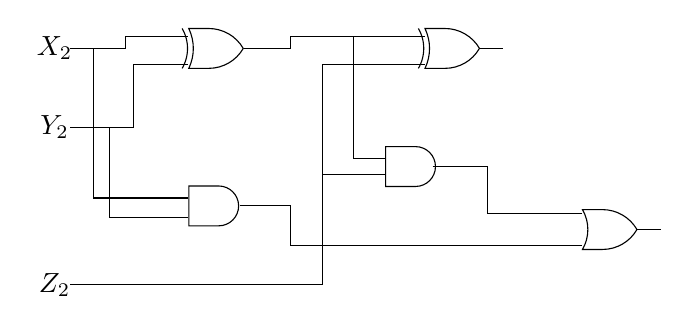
\begin{tikzpicture}[label distance=2mm]





    \node (x1) at (0,-0) {$X_2$};
    \node (x2) at (0,-1) {$Y_2$};
     \node (x3) at (0,-3) {$Z_2$};
 
    \node[and gate US, draw, rotate=0] at ($(x2)+(2,-1)$) (and1) {};
    \node[xor gate US, draw, rotate=0] at ($(x2)+(2,1)$) (xor1) {};
    \node[xor gate US, draw, rotate=0] at ($(x2)+(5,1)$) (xor2) {};
     \node[and gate US, draw, rotate=0] at ($(x2)+(4.5,-0.5)$) (and2) {};
      \node[or gate US, draw, rotate=0] at ($(x2)+(7,-1.3)$) (or1) {};
    \draw (0.2,0)--(0.5,0);
  \draw(0.5,0)--(0.9,0)--(0.9,0.15)--(1.7,0.15);
  \draw (0.2,-1)--(0.5,-1);
  \draw (0.5,-1)--(1,-1)--(1,-0.2)--(1.7,-0.2);
  \draw (0.5,0)--(0.5,-1.9)--(1.7,-1.9);
  \draw (0.7,-1)--(0.7,-2.15)--(1.7,-2.15);
  \draw (2.4,-0)--(3,-0);
   \draw(3,-0)--(3,0.15)--(4.7,0.15);
   \draw (0.2,-3)--(3.4,-3)--(3.4,-0.2)--(4.7,-0.2);
   \draw (2.35,-2)--(3,-2);
   \draw (3,-2)--(3,-2.5)--(6.7,-2.5);
   \draw (3.4,-1.6)--(4.2,-1.6);
   \draw (3.8,0.15)--(3.8,-1.4)--(4.2,-1.4);
   \draw (4.8,-1.5)--(5.5,-1.5);
   \draw (5.5,-1.5)--(5.5,-2.1)--(6.7,-2.1);
   \draw (5.4,0)--(5.7,0);
   \draw(7.4,-2.3)--(7.7,-2.3);
   
\end{tikzpicture}
\end{document}    
   
   

 

